%\documentclass[]{article}
\documentclass[7.5pt,twocolumn]{article}
\usepackage[a4paper, margin=0.8in]{geometry}
\usepackage{enumerate}
\usepackage[shortlabels]{enumitem}
\usepackage{amsmath}
\usepackage{amssymb}
\usepackage{amsfonts} 
\usepackage{graphicx}
\graphicspath{ {./images/} }
\usepackage[table]{xcolor}
\usepackage{tikz}
\usepackage{float}
\usepackage{siunitx}
\usepackage{pgfplots}
\usepackage{multirow}
\usepackage{blindtext}
\pgfplotsset{width=10cm,compat=1.9}
\usetikzlibrary{trees}
\usetikzlibrary{arrows.meta, automata,
	calc,
	positioning,
	quotes,
	shapes}
\usepackage{enumerate}
\usepackage[shortlabels]{enumitem}
\usepackage{listing}
\usepackage{color}
\usepackage{listings}
\usepackage{csquotes}
\usepackage{hyperref}
\usepackage{enumerate}
\usepackage{graphicx}
\usepackage{listings}
\usepackage{caption}
\usepackage{subcaption}
\usepackage{amsmath}
\usepackage{amssymb}
\usepackage[table]{xcolor}
\usepackage{pdflscape}
\usepackage{float}
\usepackage{siunitx}
\usepackage{chngpage}
\hypersetup{
	colorlinks=true,
	linkcolor=blue,
	filecolor=magenta,
	urlcolor=cyan,
	pdftitle={Overleaf Example},
	pdfpagemode=FullScreen,
}



\usepackage[
backend=biber,
sorting=none,
style=ieee,
]{biblatex}

\addbibresource{references.bib} %Imports bibliography file

\usepackage{mathtools}
\usepackage{xcolor}

\definecolor{codegreen}{rgb}{0,0.6,0}
\definecolor{codegray}{rgb}{0.5,0.5,0.5}
\definecolor{codepurple}{rgb}{0.58,0,0.82}
\definecolor{backcolour}{rgb}{0.99,0.99,0.99}
\definecolor{commentgray}{rgb}{0.6,0.6,0.6}

\newcommand{\verteq}{\rotatebox{90}{$\,=$}}
\newcommand{\equalto}[2]{\underset{\scriptstyle\overset{\mkern4mu\verteq}{#2}}{#1}}

\urlstyle{same}
\renewcommand{\thesection}{Part \arabic{section}}
\lstdefinestyle{mystyle}{
	backgroundcolor=\color{backcolour},   
	commentstyle=\color{commentgray},
	keywordstyle=\color{magenta},
	numberstyle=\tiny\color{codegray},
	stringstyle=\color{codepurple},
	basicstyle=\ttfamily\footnotesize\bfseries,
	breakatwhitespace=false,
	breaklines=true,
	captionpos=t,
	keepspaces=true,
	numbers=left,
	numbersep=5pt,
	showspaces=false,
	showstringspaces=false,
	showtabs=false,
	tabsize=4
}% -- Setting up the custom style
\lstset{
	style=mystyle,
	framexleftmargin=3.5mm,
	frame=shadowbox,
	rulesepcolor=\color{black},
	linewidth=\linewidth,
	xleftmargin=12pt,
	aboveskip=12pt,
	belowskip=12pt
}
\usepackage{sectsty}

\sectionfont{\fontsize{12}{15}\selectfont}

\usepackage{multicol}
\setlength{\columnsep}{1cm}

%opening
\title{Research Proposal: Machine Learning for Emotion Unveiling in a multidimensional World}
\author{Alan Teesdale\\{\small Supervisors: Qi Chen, Bing Xue}}


\begin{document}
	\maketitle
	\section{Problem Statement}
	
	The problem of Facial Expression Recognition (FER) is a classic task for computer vision, where the aim is to take an image of a person and produce and be able to learn to recognise the expression on their face. These can be broadly catagorised into two buckets. The discrete/categorical models, where emotions are divided into discrete categories (happy, sad, surprised, tired, \dots), and dimensional models, where emotions are represented on a continuous spectrum. One such model is the circumplex model\supercite{Circumplex} where emotions are represent by two values Valence, how positive the emotion is, and Arousal, how intense the emotion is.
	\begin{figure}[H]
		\centering
		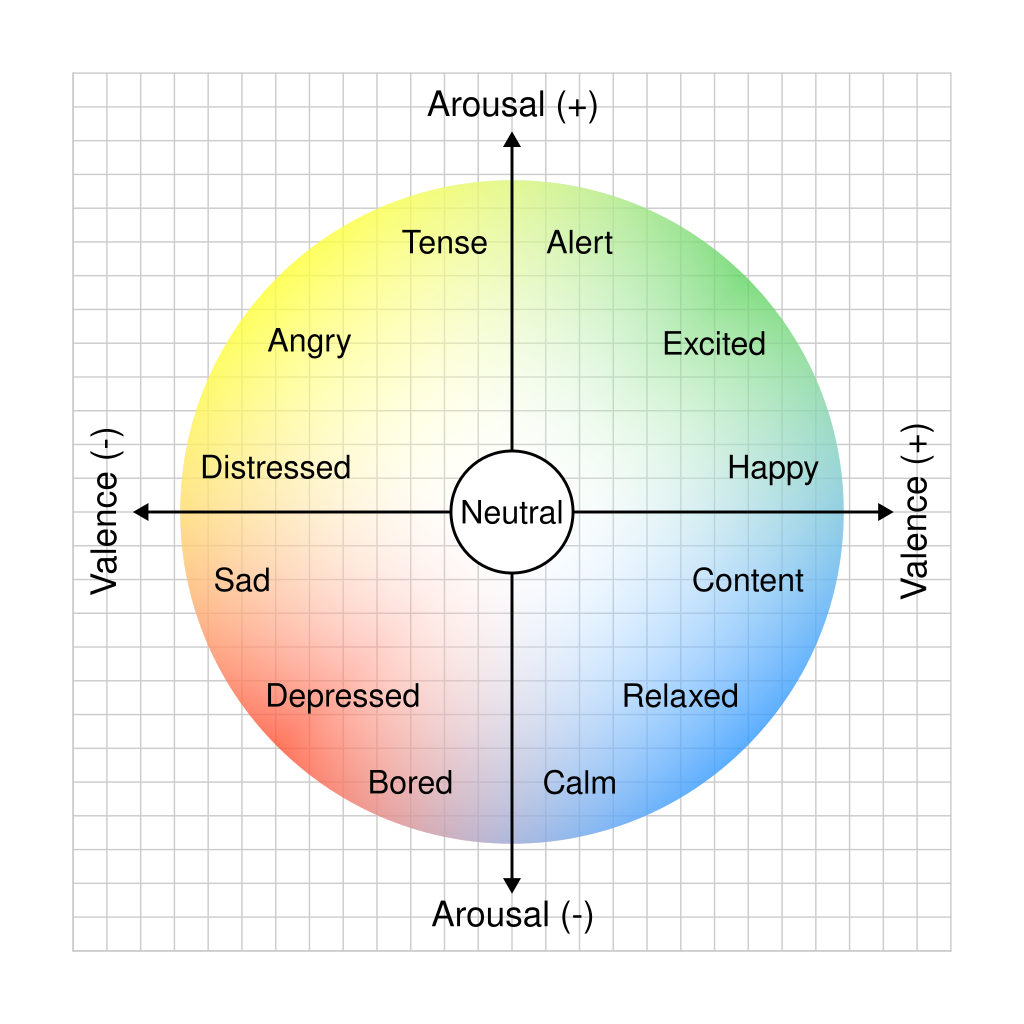
\includegraphics[width=0.8\linewidth]{Circumplex_model_of_emotion}
		\caption{A figure depicting the circumplex model. Image taken from wikimedia\supercite{wiki:img}}
		\label{fig:circumplexmodelofemotion}
	\end{figure}
	For this project we aim to use a Genetic Programming approach to construct a human interpretable model to take a to take an image of a face and convert and extract the valance and arousal corresponding to the facial expression.
	\section{Motivation}
	% why do we care?
	Facial expressions is an incredibly powerful methods of human subconscious communication, allowing machine systems to sense and change behaviour based on the emotions of the user could allow for new\footnote{and potentially dystopian} types of machine human interaction and potentially smooth out others that already exist. Because of this an other reasons, FER is a classic task in computer vision that has been studied for many decades\supercite{history}.\\
	% limitations of existing methods
	Since the field of FER is so mature, many models have been developed for this task (although the majority of the work focuses on categorical models, which by it's nature can struggle to capture mixed emotions), including similar GP models\supercite{exampleGP}.
	% PROOF READ AFTER THIS
	However, a historical constraint of many of these models is the available training data, as historically the photos are often taken in laboratory conditions, well lit, posed, or are of smaller datasets\supercite{Mollahosseini_2019}. Both of these effects mean that these models tend to do much worse ``in the wild'' where the data is ``messier'' (variable lighting, faces at different angles, e.t.c.). To address these concerns \emph{AffectNet}\supercite{Mollahosseini_2019} was created, a database with more than 1 million faces in these ``messier'' conditions. In this project we will use the \emph{AffectNet} dataset to train a new FER model that will hopefully be able handle the variable conditions needed to FER ``in the wild''.\\
	
	The preferred model in literature appears to be CNN based methods\supercite{survey}, as they often provide very good results in practice. However, the explainability of these models is very poor, especially with deep CNN's, so often these models get treated like black boxes. GP methods have been used\supercite{JAFFE_GP} for similar tasks, with comparable results to other models, including CNN based methods.\\
	% why this method solves that gap
	While there has been use of GP for similar tasks, the use of GP based models on the \emph{AffectNet} dataset is seemingly unexplore,d, and GP based models that predict dimensional models. In this project we aim to extend the use GP models for FER to use the \emph{AffectNet} database and to predict the values for arousal and valence. We hope to achieve the following:
	% Three research objectives
	\begin{enumerate}
		\item Use genetic programming to create a reasonably simple and explainable FER model
		\item Maintain roughly comparable performance to current CNN models
		\item Find a minimal but effective function set, so that the training time is reduced.
	\end{enumerate}
	\section{How?}
	To achieve this we will use Strongly typed GP to enable us to create a multi-layered GP model where we have layers corresponding to different tasks. Figure \ref{fig:examplemodel} depicts what a model might look like. The first layer represents the inputs to the system, where the image is given by the user and the other constants are evolved throughout the running of the program. The second layer takes these inputs and converts them into regions of interest, the third layer takes these regions and transforms them into a numerical feature (an example might take a Region R run it through a transformation to pull out the edges, then finally get the std of that to convert it to a number). The fourth layer takes takes the numbers produced by the previous layer and operates on those number (scaling, division, addition, subtraction...) till only 2 values remain. These two values are combined in the 5th layer into a pair and then outputted as the final result.
	\begin{figure}[H]
		\centering
		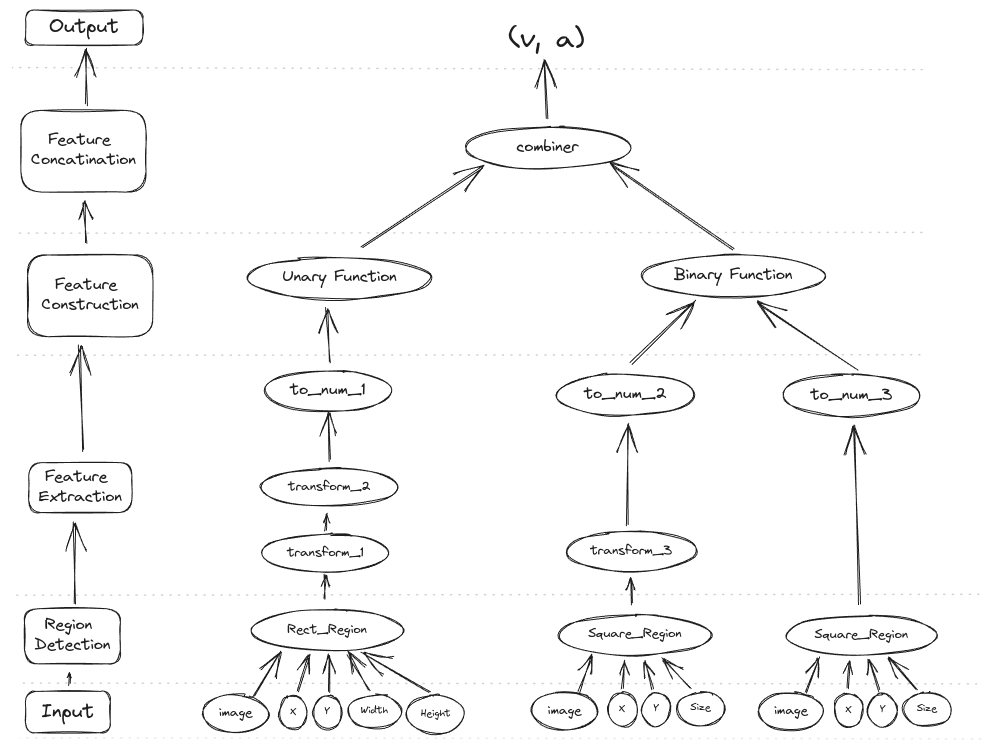
\includegraphics[width=\linewidth]{example_model}
		\caption{An example of what a tree generated by this program could look like. Image and general architecture inspired by\supercite{GPIC}}
		\label{fig:examplemodel}
	\end{figure}
	
	\section{Milestones}
	The Plan of this project will hopefully be something like the following:
	\begin{itemize}
		\item Research related work.
		\item Implement simple models.
		\item Implement more complex and powerful GP models.
		\item Increase the complexity of the function set.
		\item Decide on most effective model (taking into account accuracy and complexity of produced models).
		\item See if the complexity of the models/function set can be reduced without impacting the performance too much.
		\item Compare to existing models.
	\end{itemize}
	\section{Resources}
	The resources needed for this project should be pretty light, training the GP models could be computationally expensive, especially if lots of runs with different function sets to determine are needed to good function sets.
	\printbibliography{}
\end{document}